\documentclass[tikz]{standalone}
\usepackage{tikz}
\usepackage{amssymb}

\usetikzlibrary{shapes,arrows,positioning, calc, fit, decorations.pathreplacing}



\begin{document}

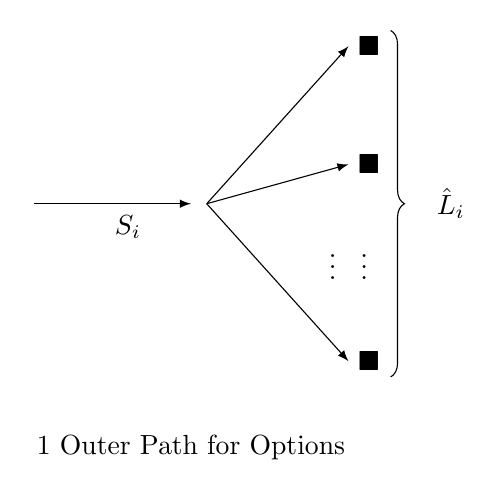
\begin{tikzpicture}[scale=1]
    \draw[-latex] (0,0)--(2,0);
    \draw[-latex] (2.2,0)--(4,2) node[right]  {$\blacksquare$};
    \draw[-latex] (2.2,0)--(4,0.5) node[right]  {$\blacksquare$};
    \draw[-latex] (2.2,0)--(4,-2) node[right]  {$\blacksquare$};
    \node at (1.2,-0.3) {$S_i$};
    \node at (3.8,-0.7) {$\vdots$};
    \node at (4.2,-0.7) {$\vdots$};
    \draw [decorate,  decoration = {brace,    raise=1pt,    amplitude=5pt}] (4.5,2.2) --  (4.5,-2.2);
    \node at (5.3,0) {$\hat L_i$};
    \node at (2,-3.1) {1 Outer Path for Options};
\end{tikzpicture}

\end{document}